\section{第五章\quad 气体和蒸汽的基本热力过程}

% 1到4节

\pt{多变过程}：满足 $p v^n=\mathrm{const.}$ 且 $n=\mathrm{const.}$ 的可逆过程称为多变过程，$n$ 称为\pt{多变指数}。$n=0$：$p=\mathrm{const.}$
为定压过程；$n=1$：$p v=\mathrm{const.}$，对理想气体，表示定温过程；$n=\kappa$：$p v^\kappa=\mathrm{const.}$，表示定熵过程，也就是可逆绝热过程；$n=\pm\infty$：$v=\mathrm{const.}$，定容过程。

{\renewcommand{\arraystretch}{1.18}
\setlength{\tabcolsep}{1.2pt}
\resizebox{\linewidth}{!}{%
    \begin{tabular}{|c|c|c|c|c|c|}
        \hline
         & 定容 $n=\infty$             & 定压 $n=0$ & 定温 $n=1$ & 定熵 $n=\kappa$ & 多变 $n$ \\
        \hline
        特征
         & $v=\mathrm{const.}$
         & $p=\mathrm{const.}$
         & $T=\mathrm{const.}$
         & $s=\mathrm{const.}$
         & $pv^n=\mathrm{const.}$                                                   \\
        \hline
        $T,p,v$ 关系
         &
        $\frac{T_1}{p_1}=\frac{T_2}{p_2}$
         &
        $\frac{T_1}{v_1}=\frac{T_2}{v_2}$
         &
        $p_1v_1=p_2v_2$
         &
        $\begin{gathered}
                 p_1v_1^\kappa=p_2v_2^\kappa\\
                 T_1v_1^{\kappa-1}=T_2v_2^{\kappa-1}\\
                 T_1p_1^{-(\kappa-1)/\kappa}
                 =T_2p_2^{-(\kappa-1)/\kappa}
             \end{gathered}$
         &
        $\begin{gathered}
                 p_1v_1^n=p_2v_2^n\\
                 T_1v_1^{n-1}=T_2v_2^{n-1}\\
                 T_1p_1^{-(n-1)/n}
                 =T_2p_2^{-(n-1)/n}
             \end{gathered}$                                                   \\
        \hline
        $\Delta u$
         & $c_{\mathrm{V}}(T_2-T_1)$
         & $c_{\mathrm{V}}(T_2-T_1)$
         & $0$
         & $c_{\mathrm{V}}(T_2-T_1)$
         & $c_{\mathrm{V}}(T_2-T_1)$                                                \\
        \hline
        $\Delta h$
         & $c_p(T_2-T_1)$
         & $c_p(T_2-T_1)$
         & $0$
         & $c_p(T_2-T_1)$
         & $c_p(T_2-T_1)$                                                           \\
        \hline
        $\Delta s$
         &
        $c_{\mathrm{V}}\ln\frac{T_2}{T_1}$
         &
        $c_p\ln\frac{T_2}{T_1}$
         &
        $\begin{gathered}
                 \frac{q}{T}\\
                 R_{\mathrm{g}}\ln\frac{v_2}{v_1}\\
                 R_{\mathrm{g}}\ln\frac{p_1}{p_2}
             \end{gathered}$
         &
        $0$
         &
        $\begin{gathered}
                 c_{\mathrm{V}}\ln\frac{T_2}{T_1}
                 +R_{\mathrm{g}}\ln\frac{v_2}{v_1}\\
                 c_p\ln\frac{T_2}{T_1}
                 -R_{\mathrm{g}}\ln\frac{p_2}{p_1}\\
                 c_{\mathrm{V}}\ln\frac{p_2}{p_1}
                 +c_p\ln\frac{v_2}{v_1}
             \end{gathered}$                               \\
        \hline
        比热容 $c$
         &
        $c_{\mathrm{V}}=\frac{R_{\mathrm{g}}}{\kappa-1}$
         &
        $c_p=\frac{\kappa R_{\mathrm{g}}}{\kappa-1}$
         &
        $\infty$
         &
        $0$
         &
        $c_n=\frac{n-\kappa}{n-1}c_{\mathrm{V}}$                                    \\
        \hline
        过程功 $w$
         &
        $0$
         &
        $\begin{gathered}
                 p(v_2-v_1)\\
                 R_{\mathrm{g}}(T_2-T_1)
             \end{gathered}$
         &
        $\begin{gathered}
                 R_{\mathrm{g}}T\ln\frac{v_2}{v_1}\\
                 R_{\mathrm{g}}T\ln\frac{p_1}{p_2}
             \end{gathered}$
         &
        $\begin{gathered}
                 -\Delta u\\
                 \frac{R_{\mathrm{g}}}{\kappa-1}(T_1-T_2)\\
                 \frac{R_{\mathrm{g}}T_1}{\kappa-1}
                 \left[1-\left(\frac{p_2}{p_1}\right)^{(\kappa-1)/\kappa}\right]
             \end{gathered}$
         &
        $\begin{gathered}
                 \frac{R_{\mathrm{g}}}{n-1}(T_1-T_2)\\
                 \frac{R_{\mathrm{g}}T_1}{n-1}
                 \left[1-\left(\frac{p_2}{p_1}\right)^{(n-1)/n}\right]
             \end{gathered}$                          \\
        \hline
        技术功 $w_{\mathrm{t}}$
         &
        $v(p_1-p_2)$
         &
        $0$
         &
        $w_{\mathrm{t}}=w$
         &
        $\begin{gathered}
                 -\Delta h\\
                 \frac{\kappa R_{\mathrm{g}}}{\kappa-1}(T_1-T_2)\\
                 \frac{\kappa R_{\mathrm{g}}T_1}{\kappa-1}
                 \left[1-\left(\frac{p_2}{p_1}\right)^{(\kappa-1)/\kappa}\right]\\
                 w_{\mathrm{t}}=\kappa w
             \end{gathered}$
         &
        $\begin{gathered}
                 \frac{nR_{\mathrm{g}}}{n-1}(T_1-T_2)\\
                 \frac{nR_{\mathrm{g}}T_1}{n-1}
                 \left[1-\left(\frac{p_2}{p_1}\right)^{(n-1)/n}\right]\\
                 w_{\mathrm{t}}=nw
             \end{gathered}$                         \\
        \hline
        过程热量 $q$
         &
        $\Delta u$
         &
        $\Delta h$
         &
        $\begin{gathered}
                 T(s_2-s_1)\\
                 q=w=w_{\mathrm{t}}
             \end{gathered}$
         &
        $0$
         &
        $\frac{n-\kappa}{n-1}c_{\mathrm{V}}(T_2-T_1)$                               \\
        \hline
    \end{tabular}%
}}

\divider

\noindent
\begin{minipage}[t]{0.48\linewidth}
    \vspace{0pt}
    若经历水加热、汽化、过热三个阶段：
    \pt{液体加热量}：$q_l=h_1-h_0$；\pt{汽化潜热}：$\gamma=h_2-h_1$；\pt{过热热量}：$q_{\mathrm{sup}}=h_3-h_2$；\pt{总定压换热量}：$q_p=h_3-h_0$； 汽化潜热随压力升高而减小
\end{minipage}
\hfill
\begin{minipage}[t]{0.48\linewidth}
    \vspace{0pt}
    \centering
    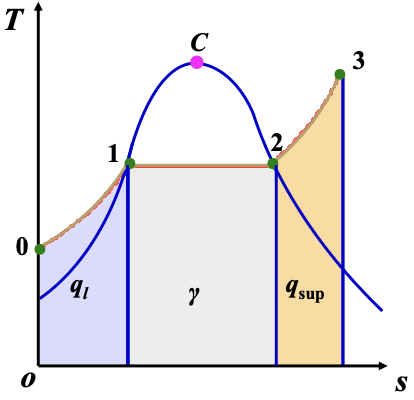
\includegraphics[width=0.8\linewidth]{figures/5水加热的ts图.png}
\end{minipage}

\divider